\documentclass[10pt]{beamer}
\usepackage{csquotes}% Recommended

\usepackage{graphicx}
\usepackage{xcolor}
\usepackage{amsfonts}
\usepackage{amsmath}
\usepackage{amssymb}
\usepackage[skip=10pt plus1pt] {parskip}


%Information to be included in the title page:
\title{Multivariable Calculus}
\author{UChicago Political Science Math Camp}
\institute{Ryan Gibbons \& Luke Cain}
\date{2025}

\begin{document}

\frame{\titlepage}

\begin{frame}{Multivariable Calculus}

Really, it's not that bad
    \begin{itemize}
        \item this is very true for derivatives
        \item this is kind of true for integrals
    \end{itemize}
\end{frame}

\begin{frame}{Functions}
    Recall our definition of a \textbf{function}: \\

    \vspace{1cm}

    \begin{quote}
        A function is a mapping of elements in some set to elements in another set.
    \end{quote}

    So far, we have been working with functions of the form:

    \[f: \mathbb{R} \rightarrow \mathbb{R}\]

    which we simplify into $f: x \rightarrow f(x)$ or $f: x \rightarrow y$.
\end{frame}

\begin{frame}{Multivariable Functions}
    Multivariable functions\footnote{to the extent that we are concerned about them} return an output given a series of inputs. More generally, we examine:

    \[f: \mathbb{R}^n \rightarrow \mathbb{R}\]

    Such that we ``blend" $n$ input numbers into a single output $f(x_1,x_2,...,x_n)$ \\

    \vspace{1cm}
    \textcolor{red}{This is not visually interpretable beyond $n=2$.}
\end{frame}

\begin{frame}{Example}
We can represent the following as multivariate functions:

\begin{itemize}
        \item The \textbf{wind chill} $W_c$ is a function of temperature $t$ and wind speed $s$
        \item Your \textbf{commute time} (from Pick, walking) $C$ is a function of your numbered street $n$, cross street $s$, and walking speed $w$
        \item Your \textbf{grocery store bill} $G$ is a function of price $p_i$ and quantity $q_i$ for each product $i \in \{\text{shopping list}\}$
    \end{itemize}
\end{frame}

\begin{frame}{Recap: Hints for Multivariable Functions}
\begin{itemize}
    \item Hint \#1: use $\mathbb{R}^n$ for $n$ input variables
    \item Hint \#2: we are often just mapping something onto $\mathbb{R}$, which means that for the input(s), \textit{we just recover a single numeric output.}
    \item Hint \#3: don't try to visualize functions involving beyond $\mathbb{R}^3$ (and really not beyond $\mathbb{R}^2$)
\end{itemize}
\end{frame}

\begin{frame}{Multivariable Calculus}
    calls for two expansions of our existing toolbox:

    \begin{enumerate}
        \item Partial derivation
        \item Iterated integration
    \end{enumerate}

Both will take a common approach: \textit{treat non-w.r.t. variables as constants!}
\end{frame}

\begin{frame}{Partial Derivatives: Step 1}
    \begin{center}
        \includegraphics[width=10cm]{leversjpeg.jpg}
    \end{center}
\end{frame}

\begin{frame}{Partial Derivatives: Step 2}
    \begin{center}
        \includegraphics[width=10cm]{guage.jpg}
    \end{center}
\end{frame}

\begin{frame}{Partial Derivatives}
    \textit{What happens to the gauge when you move one (1) lever?} \\

    \vspace{.5cm}
    This is contingent on two primary things:
    \begin{enumerate}
        \item What direction you move that lever
        \item Where all the other levers are set
    \end{enumerate}
\vspace{1cm}
    \textcolor{red}{These conditions are re-evaluated \textbf{\underline{at every point!}}}
\end{frame}

\begin{frame}{Notation}
    We use the $\partial$ symbol to represent a partial derivative:

    \[\frac{\partial f}{\partial a}\]
    
    represents the \textbf{instantaneous rate of change} of $f$, given a change in \textit{only} $a$. To take a second derivative, we use

    \[\frac{\partial ^2 f}{\partial a^2}\]

    Why can't we use $f'$ as notation?
\end{frame}

\begin{frame}{How We Do It}
    To take a partial derivative, we follow simple steps:

    \begin{enumerate}
        \item Identify the variable of derivation:
        \[\frac{\partial f}{\partial a} \bigg[2a^2 + a^3b\bigg]= \text{partial of $f$ w.r.t $a$}\]
        \item Treat all other variables (i.e., $b$) as constants, then follow normal derivation rules for $a$: \pause
        \[\implies2 \cdot a^{2-1} +  b \cdot 3 \cdot a^2\]
        \[\implies \frac{\partial f}{\partial a} = 4a + 3ba^2 \textcolor{red}{= a(4 + 3ba)}\]
    \end{enumerate}

    Recall that the derivative of a constant is $0$, so $\frac{\partial f}{\partial a}$ for a term excluding $a$ is $0$.
\end{frame}

\begin{frame}{Some Evaluation}
    We've recovered

    \[\frac{\partial}{\partial a} \bigg[ 2a^2 + a^3b\bigg] = a(4 + 3ba)\]

    What does this tell us about $f$ with respect to $a$? \\

    \vspace{1cm}
    \pause

    Now, let's calculate $\frac{\partial f}{\partial b}$. What does this tell us about $f$ with respect to $b$?
\end{frame}

\begin{frame}{Some More Examples}
    The exact same is true no matter how many terms. For example, solve $\frac{\partial}{\partial k}$ for each $k$ in the following:

    \[ 2xy^2 + 2x^2y + xy\]

    \[3(xy)^2 + \frac{1}{w(x+y)}\]

    \[\sqrt{xy} + x^2 y^2 + e^{2w}\]

    In this way, we can fully characterize each partial derivative
\end{frame}

\begin{frame}{A Grounding Moment}
    \begin{center}
        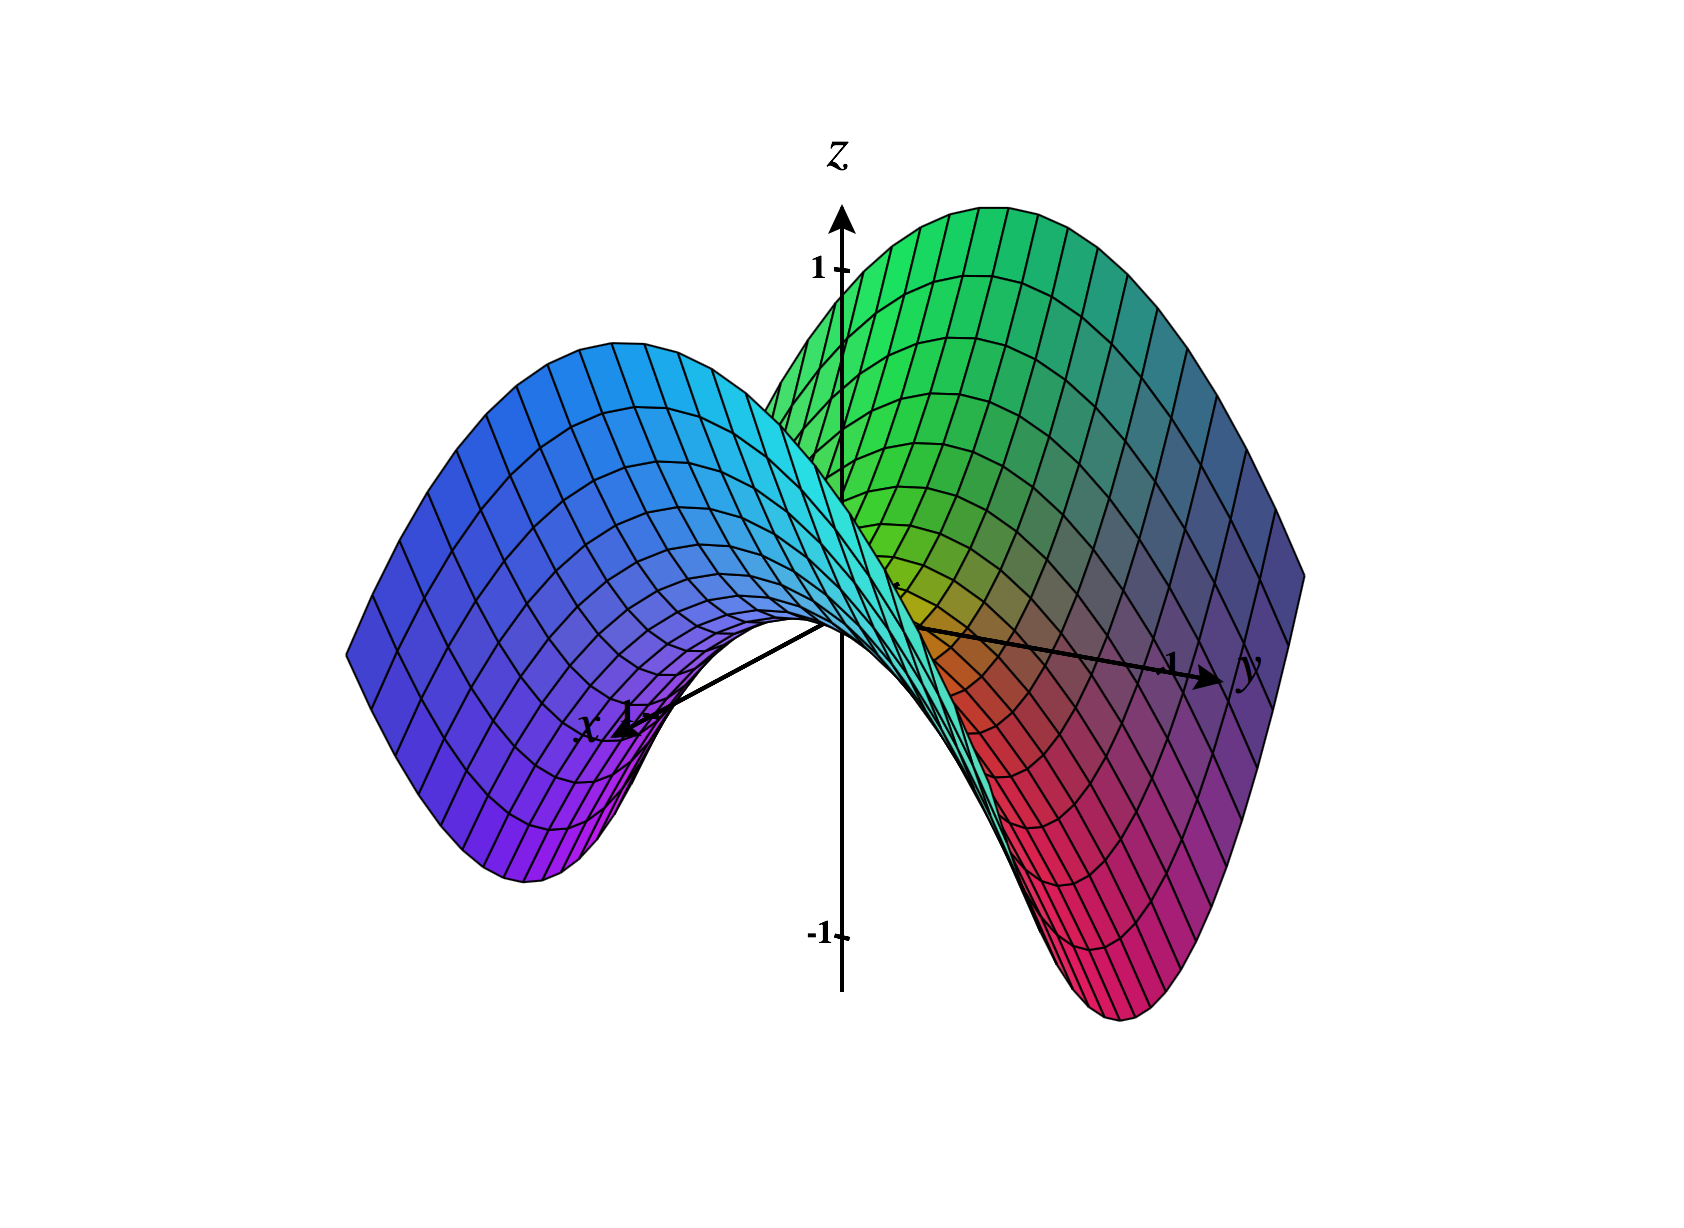
\includegraphics[width = 10cm]{CalcPlot3D-hyper_para2.png}
    \end{center}
\end{frame}

\begin{frame}{Cross Derivative}
    We can take a second derivative using this same process, just repeated. We can also take a \textbf{cross derivative}, taking a partial of one variable and then a partial of that result:

    \[\frac{\partial^2 f}{\partial y \partial x} = \frac{\partial}{\partial y} \bigg[ \frac{\partial f}{\partial x}\bigg]\]

    \textit{How the derivative of $f$ with respect to $x$ changes with respect to $y$}
\end{frame}

\begin{frame}{Multivariable Optimization}
    If we are just optimizing a multivariable function w.r.t. one variable, we calculate the first order condition for that variable, and compare to endpoints (this is most common) \\

    \vspace{1cm}

    Otherwise, we exploit the same logic: what would $\frac{\partial f}{\partial k} \neq 0$ imply for any $k$?
\end{frame}

\begin{frame}{Critical Points}
Just like single-variable functions, we begin with \textbf{critical points} where $\frac{\partial f}{\partial k} = 0$ \\

\vspace{.5cm}

But, we extend this: it must be true that $\frac{\partial f}{\partial k} = 0 \; \forall \; k$...

\vspace{.5cm}

We often get a \textbf{system of equations}
\end{frame}

\begin{frame}{Systems of Equations}
    Given a series of equalities (or inequalities), we must satisfy \underline{all} of them. We can use \\

    \begin{enumerate}
        \item Substitution -- isolate for one variable, plug into others
        \item Addition/subtraction (messy)
        \item Computation
    \end{enumerate}
\end{frame}

\begin{frame}{An Example}
    Take from above:

    \[f(x,y) = 2xy^2 + 2x^2y + xy\]

    What are our critical points? \\ \pause

    \vspace{.5cm}
    Solve for partial derivatives:
    \[\frac{\partial f}{\partial x} = 2y^2 + 4xy + y = y(2y + 4x + 1)\]
    \[\frac{\partial f}{\partial y} = 4xy + 2x^2 + x = x(2x + 4y + 1)\]
    When are both of these equal to zero?
\end{frame}

\begin{frame}{An Example}
    \[y(2y + 4x + 1) = 0 \iff y \in \{0,\frac{-4x-1}{2}\}\]
    \[x(2x + 4y + 1) = 0 \iff x \in \{0, \frac{-4y-1}{2}\}\]

    This yields four combinations:

    \[(x^*, y^*) \in \bigg\{\Big(0,0\Big), \Big(\frac{-4y-1}{2},0\Big), \Big(0,\frac{-4x-1}{2}\Big),\Big(\frac{-4x-1}{2}, \frac{-4y-1}{2}\Big) \bigg\}\]
    For our internal points, we have the other variable: $y = x = \frac{-1}{2}$. Then, we solve our system of equations, to recover our critical points
    \[(x^*, y^*) \in \bigg\{\Big(0,0\Big), \Big(\frac{-1}{2},0\Big), \Big(0,\frac{-1}{2}\Big),\Big(\frac{-1}{6}, \frac{-1}{6}\Big) \bigg\}\]
\end{frame}

\begin{frame}{End Points}
    Both of our partial derivatives are strictly increasing in their variables, so we also examine the points at $(\pm \infty, \pm \infty)$:

    \[f(\infty, \infty) = \infty\]
    \[f(\infty, -\infty) = \text{undefined}\]
    \[f(-\infty,-\infty) = \infty\]
    \[f(-\infty, \infty) = \text{underfined}\]

    Therefore, maxima are at $(\infty, \infty)$ and $(-\infty, -\infty)$
\end{frame}

\begin{frame}{What about minima?}
    Let's discard our end points here (I didn't think about them when choosing this function), and evaluate every critical point:

    \[f(0,0) =\]
    \[f(\frac{-1}{2},0) =\]
    \[f(0, \frac{-1}{2}) =\]
    \[f(\frac{-1}{6},\frac{-1}{6}) = \]

    The minima of $f$ is therefore at the lowest-value critical point here.
\end{frame}

\begin{frame}{Multivariate Integration}
    Integration of a multivariable function works just like a partial derivative:

    \begin{enumerate}
        \item Identify the variable of integration:
        \[\int 2a^2 + a^3b \; da = \text{Integration of $f(a,b)$ over $a$}\]
        \item Treat all other variables (i.e., $b$) as constants, then follow normal derivation rules for $a$:
        \[\implies \frac{2a^{2+1}}{2+1} + \frac{ba^{3+1}}{3+1}\]
        \[\implies \int f(a,b) \; da = \frac{2a^3}{3} + \frac{ab^4}{4}\]
    \end{enumerate}
    Recall that the integral of $k$ over a constant $m$ is $k\cdot m$, so $\int f\; da = f \cdot a$ for a term excluding $a$.
\end{frame}

\begin{frame}{Some More Examples}
    Solve $\int f \: dk$ for each $k$ in the following:

    \[2xy^2 + 2x^2y + xy\]

    \[3(xy)^2 + \frac{1}{wxy}\]

    \[\sqrt{xy} + x^2 y^2 + e^w\]
\end{frame}

\begin{frame}{A Brief Note}
    Recall our product corollary of integration:

    \[\int b \cdot f(x) \: dx = b \cdot \int f(x) \: dx\]

    With multivariable functions, this holds:

    \[\int b \cdot f(x,y) \: dy = b \cdot \int f(x,y)\: dy\]

    We treat non-integrated variables as constants, so... \textcolor{red}{isolate whenever possible!} i.e.

    \[\int 2y x^2 + 8 y^2x \: dx  \implies 2y \cdot \int x^2 + 4yx \: dx \]
\end{frame}

\begin{frame}{Iterated Integration}
    Sometimes, we need to integrate over multiple dimensions. For $\mathbb{R}^2$, we call this \textbf{double integration}; for $\mathbb{R}^3$, \textbf{triple integration}, etc.

    \[\int \int f(x,y) \; dx dy\] \pause

    \[\underbrace{\int \underbrace{\int f(x,y) \; dx}_{\text{Step 1}} dx}_{\text{Step 2}}\]

    \textit{Hint: inside $\rightarrow$ out}

\end{frame}

\begin{frame}{Iterated Integration (Example)}
    Let $f(x,y) = \frac{1}{2}x^2y + 2xy^2$. Evaluate

    \[\int \int f(x,y) \: dx \:dy\]

    \pause
    Now, evaluate

    \[\int \int f(x,y) \: dy \:dx\]\pause

    This is called \textbf{Fubini's theorem}
\end{frame}

\begin{frame}{For Definite Boundaries}
    We can calculate a definite iterated integral just using the same steps above (just with FTOC). \\
    
    \vspace{1cm}
    Let's evaluate, for the square from $(0,0)$ to $(2,2)$, the following:

    \[\int \int 2^x + x\sqrt{y} \: dx \: dy\]

    
\end{frame}

\begin{frame}{Closing Exercise}
    The following is used by the NWS to calculate wind chill:

    \[W(t,v) = 35.74 + 0.6215t - 35.75(v^{0.16})+0.4275t(v^{0.16})\]

    You can either wear a windbreaker to decrease perceived wind speed, or a jacket to increase perceived temperature, but a lion with your name and phone number on its collar escapes from the zoo\footnote{right next to the preschool} if you wear both. Under what conditions would you want to wear one over the other? (Assume both garments are equivalently weak and only help a little.)
\end{frame}




\end{document}